\subsection{Half-Wave Rectifier:}

The {\bfseries\itshape half-wave rectifier}, "cancels" the negative voltage, and rectifies the A.C into C.C. But still, has a Voltage loss in the second semi-period as we have seen in Figure 2.1.2. \hfill \break 

Using the 100$\Omega$ resistor as $R_{L}$ and a 1N4003 diode, the circuit of the Figure 3.2.0 was assembled. 

\begin{figure}[H]
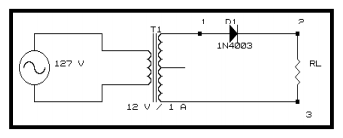
\includegraphics[scale=.8]{phalf-wave.png}
\centering \linebreak \linebreak Figure 3.2.0: Half-wave rectifier circuit.
\end{figure}

For measure the signal before being rectified, we put the positive terminal of the voltmeter in the terminal 1 of the Figure 3.2.0 and the negative terminal of the voltmeter in the terminal 3 of the Figure 3.2.0. We will call this voltage $V_{T}$ (Transformer Voltage).

\begin{ceqn}
\begin{align}
V_{T} = 13.3\ V_{rms}
\end{align}
\end{ceqn}

{\bfseries\itshape\color{OliveGreen}{Observation:}} {\bfseries\itshape\color{OliveGreen}{To measure $V_{T}$ the Voltmeter needs to be in the A.C option.}} \hfill \break

\pagebreak

In the same terminals ( 1 and 3 ), of the Figure 3.2.0, the terminals of the oscilloscope were connected same as the voltmeter. Now, as can we see in Figure 3.2.1, the signal isn't being rectified yet. To visualize the rectified signal, the terminals of the oscilloscope were connected to the terminals 2 and 3 of the Figure 3.2.0. Now, as we can see in Figure 3.2.2 the signal is rectified from A.C to D.C. Now there's no negative voltage.

\begin{multicols}{2}
\begin{figure}[H]
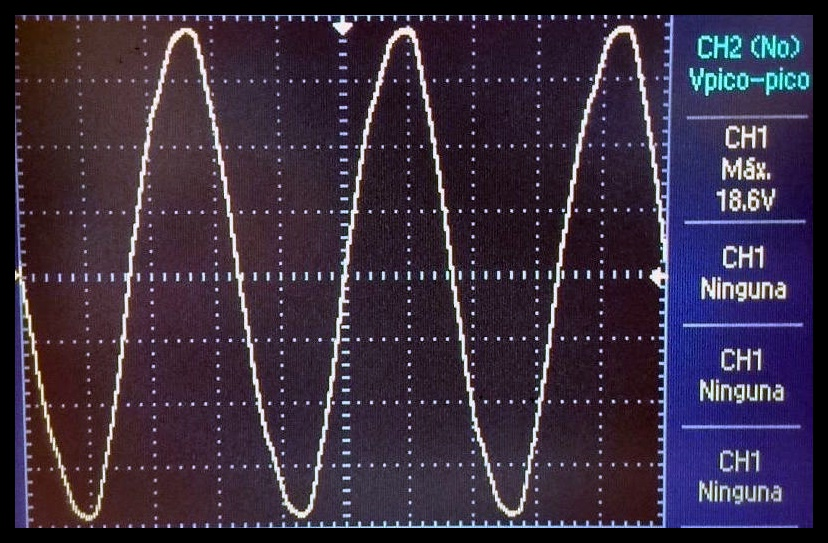
\includegraphics[scale=.25]{otransformer.jpg}
\centering \linebreak \linebreak Figure 3.2.1: Transformer output signal.
\linebreak \linebreak $\frac{5 V}{div}\ \ and\ \ \frac{5mseg}{div}$.
\end{figure}

\begin{figure}[H]
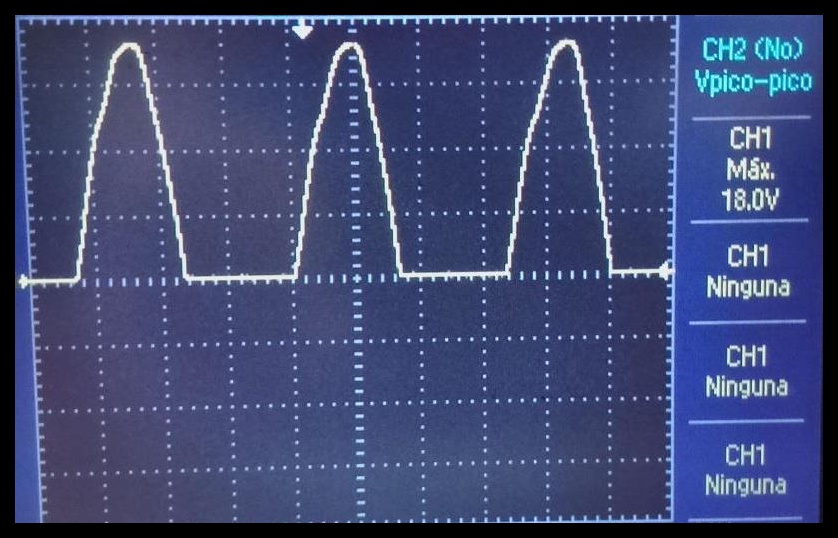
\includegraphics[scale=.25]{ohalf-wave.jpg}
\centering \linebreak \linebreak Figure 3.2.2: Half-wave rectified signal.
\linebreak \linebreak $\frac{5 V}{div}\ \ and\ \ \frac{5mseg}{div}$.
\end{figure}
\end{multicols}

{\bfseries\itshape\color{OliveGreen}{Observation:}} {\bfseries\itshape\color{OliveGreen}{In the oscilloscope we are only using the channel 1 in D.C option.}}  \hfill \break

To measure the voltage in {\bfseries\itshape $R_{L}$}, its necessary to connect the positive terminal of the voltmeter in the terminal 2 of the Figure 3.2.0 and the negative terminal of the voltmeter in the terminal 3 of the Figure 3.2.0. We will call this voltage $V_{0}$, also the resistor $R_{L}$ will have a current, we will call it $I_{0}$ and with Ohm's Law we can find it.

\begin{ceqn}
\begin{align}
V_{0} = 5.6\ V_{rms} 
\end{align}
\end{ceqn} \hfill

{\bfseries\itshape\color{OliveGreen}{Observation:}} {\bfseries\itshape\color{OliveGreen}{To measure $V_{0}$ the Voltmeter needs to be in the D.C option.}} \hfill \break \break

{\bfseries\itshape\color{Maroon}{Using Ohm's Law: $I = \frac{V}{R}.$}} \hfill \break

\begin{ceqn}
\begin{align}
I_{0} = \frac{5.6\ V_{rms}}{0.100\ \Omega} = 0.056\ A
\end{align}
\end{ceqn} \hfill 

{\bfseries\itshape
\begin{itemize}
\item For $V_{p}$ ( Peak Voltage ) of Figure 3.2.1:
\end{itemize}} 

When the terminals of the oscilloscope are connected to the circuit and the signal it's displayed on screen as Figures 3.2.1 shows. We will put the oscilloscope in the option {\bfseries\itshape measures} and search for the option {\bfseries\itshape Max Voltage}. \hfill \break

\begin{ceqn}
\begin{align}
V_{p} = 18.6 V
\end{align}
\end{ceqn} \hfill 

{\bfseries\itshape
\begin{itemize}
\item Finally, $V_{p} - V_{D}$, where $V_{p}$ it's the peak voltage in Figure 3.2.1 and $V_{D}$ it's the diode Voltage:
\end{itemize}} \hfill

\begin{ceqn}
\begin{align}
V_{p} - V_{D} = 18.6 V - 0.7 V = 17.9 V
\end{align}
\end{ceqn}

\pagebreak